\chapter{Wstęp}
\section{Wprowadzenie}
Rola automatyzacji w obsłudze klienta znacznie wzrosła w ostatnich latach. Można to zaobserwować w dynamice, z jaką ewoluują systemy informatyczne nazywane elektronicznymi biurami obsługi klienta (eBOK). Takie systemy są szeroko stosowane w różnych sektorach gospodarki, takich jak energetyka, wodociągi, telekomunikacja i usługi multimedialne. 
% TO DO: główne sektory gospodarki to: rolnictwo, przemysł, usługi. Proszę zwrócić uwagę na właściwe użycie terminów i związki frazeologiczne. 

Z punktu widzenia użytkowników główną ich zaletą eBOKów jest możliwość skorzystania z oferowanych przez nie funkcji w dowolnym miejscu i czasie. Cecha ta nie tylko poprawia jakość obsługi klienta, ale także zwiększa efektywność organizacji wdrażających takie rozwiązanie. Poza zapewnieniem dostępu do informacji o rozliczeniach i płatnościach eBOKi wspierają także realizację bardziej zaawansowanych procesów, jak zgłaszanie problemów technicznych, zarządzanie zgłoszeniami serwisowymi i~komunikację z zarządem. Ważnym aspektem tych systemów jest bezpieczeństwo danych osobowych, które jest zapewniane poprzez regularne aktualizacje systemu, wdrażanie mechanizmów uwierzytelniania dwuskładnikowego oraz zgodność z przepisami o ochronie danych osobowych, takimi jak RODO.

Obecnie na rynku spotkać można wiele systemów typu eBOK. Jednym z z nich jest system ,,Energa24''. Umożliwia on klientom dostęp do informacji o zużyciu energii, przeglądanie i pobieranie rachunków, dokonywanie płatności online oraz zgłaszanie awarii~\cite{energa}. Standardowy scenariusz dokonywania płatności za pomocą tej aplikacji pokazano na rysunku! \ref{fig:energa_manual}. Użytkownik może wybrać odpowiedni rachunek, a następnie poprzez bezpieczną bramkę płatności uiścić należności bezpośrednio w systemie.
\begin{figure}[htb]
	\centering
		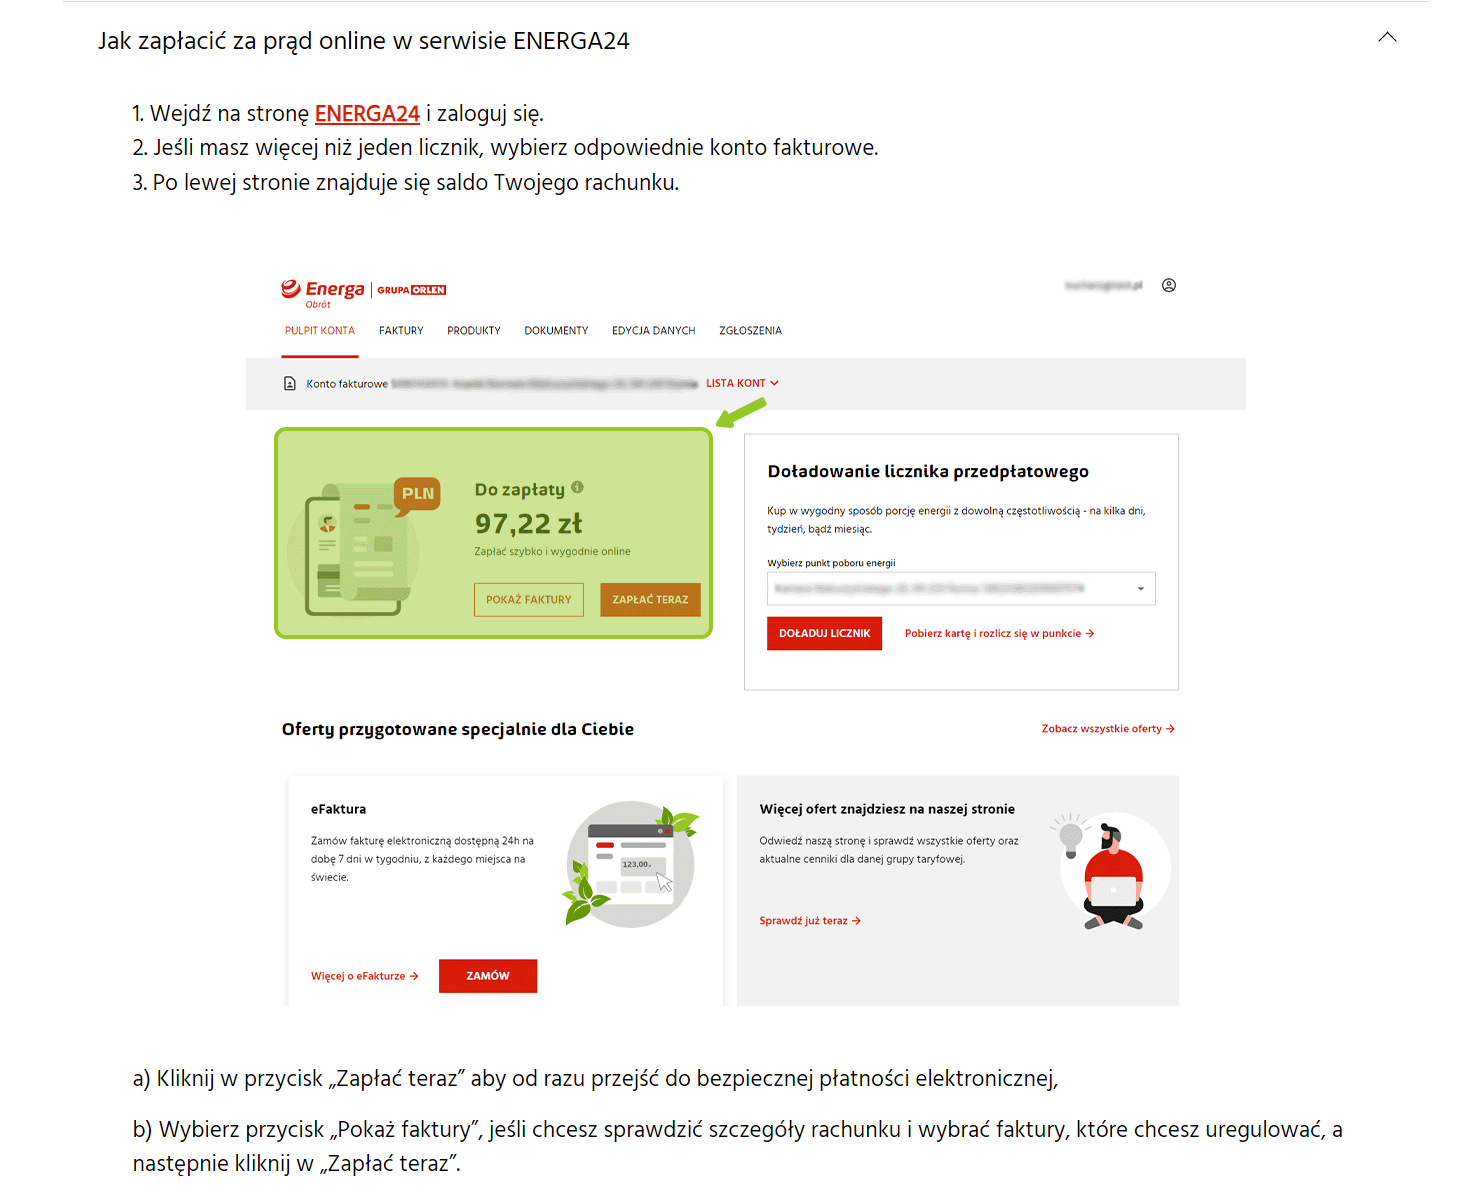
\includegraphics[width=0.85\linewidth]{zrzuty_ekranu/energa_manual_1.png} \\[-1ex]
		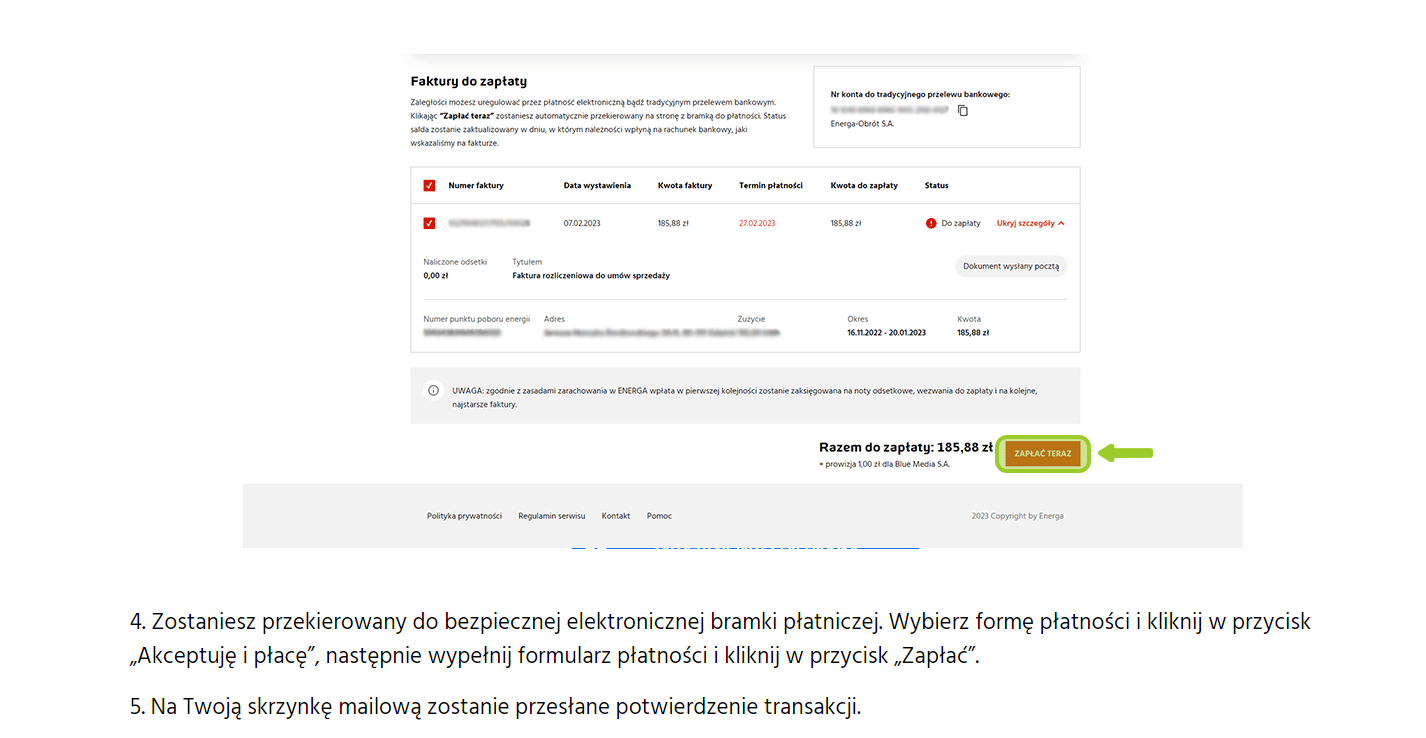
\includegraphics[width=0.85\linewidth]{zrzuty_ekranu/energa_manual_2.png} \\[-1ex]
		\caption{Opis scenariusza dokonania płatności za energię elektryczną w serwisie ,,Energa24''~\cite{energa}}
	\label{fig:energa_manual}
\end{figure}

%Innym szeroko stosowanym rozwiązaniem jest eBOK dostarczany przez Miejskie Przedsiębiorstwo Wodociągów i Kanalizacji (MPWiK) w Warszawie. Umożliwia on mieszkańcom monitorowanie zużycia wody, zarządzanie płatnościami i zgłaszanie problemów technicznych~\cite{MPWiK}.
% TO DO: dwa zdania bez rozwinięcia to trochę za mało. Taki opis nie pasuje do opisów innych przykładów wdrożeń. Proszę rozwinąć opis, albo pozostawić te zdania zamarkowane.

Dostępne są również rozwiązania dostosowane specjalnie do potrzeb spółdzielni i wspólnot mieszkaniowych. Przykładem może być system ,,e-Kartoteka'', który umożliwia mieszkańcom zarządzanie zgłoszeniami usterek oraz podgląd postępu zgłoszenia, wgląd oraz regulację w płatności za nieruchomość, wgląd w dokumenty nieruchomości oraz wspólnoty, głosowanie nad uchwałami wspólnoty, a także komunikację z zarządem~\cite{e-kartoteka}. System ten oferuje również możliwość przeglądania rozliczeń mediów, takich jak woda, energia elektryczna czy ogrzewanie, co ułatwia mieszkańcom śledzenie swoich bieżących opłat i zużycia. Aplikacja ,,e-Kartoteka'' umożliwia również mieszkańcom szybki dostęp do wyciągów z rachunków i opłat miesięcznych, w tym szczegółowych rozliczeń za media (patrz rysunek~\ref{fig:kartoteka_manual}). Dzięki intuicyjnemu interfejsowi użytkownicy mogą sprawnie poruszać się między funkcjami, takimi jak tablica ogłoszeń, forum dyskusyjne dla mieszkańców czy dokumentacja nieruchomości, co znacząco poprawia komunikację i współpracę w obrębie wspólnoty. Ponadto mieszkańcy mają możliwość zgłaszania odczytów liczników, co automatycznie generuje informacje na temat aktualnego stanu rozliczeń oraz zaległych opłat, podobnie jak widoczne na przedstawionym obrazie funkcje raportowania stanu liczników i przeglądania historii faktur.
\begin{figure}[htb]
    \centering
    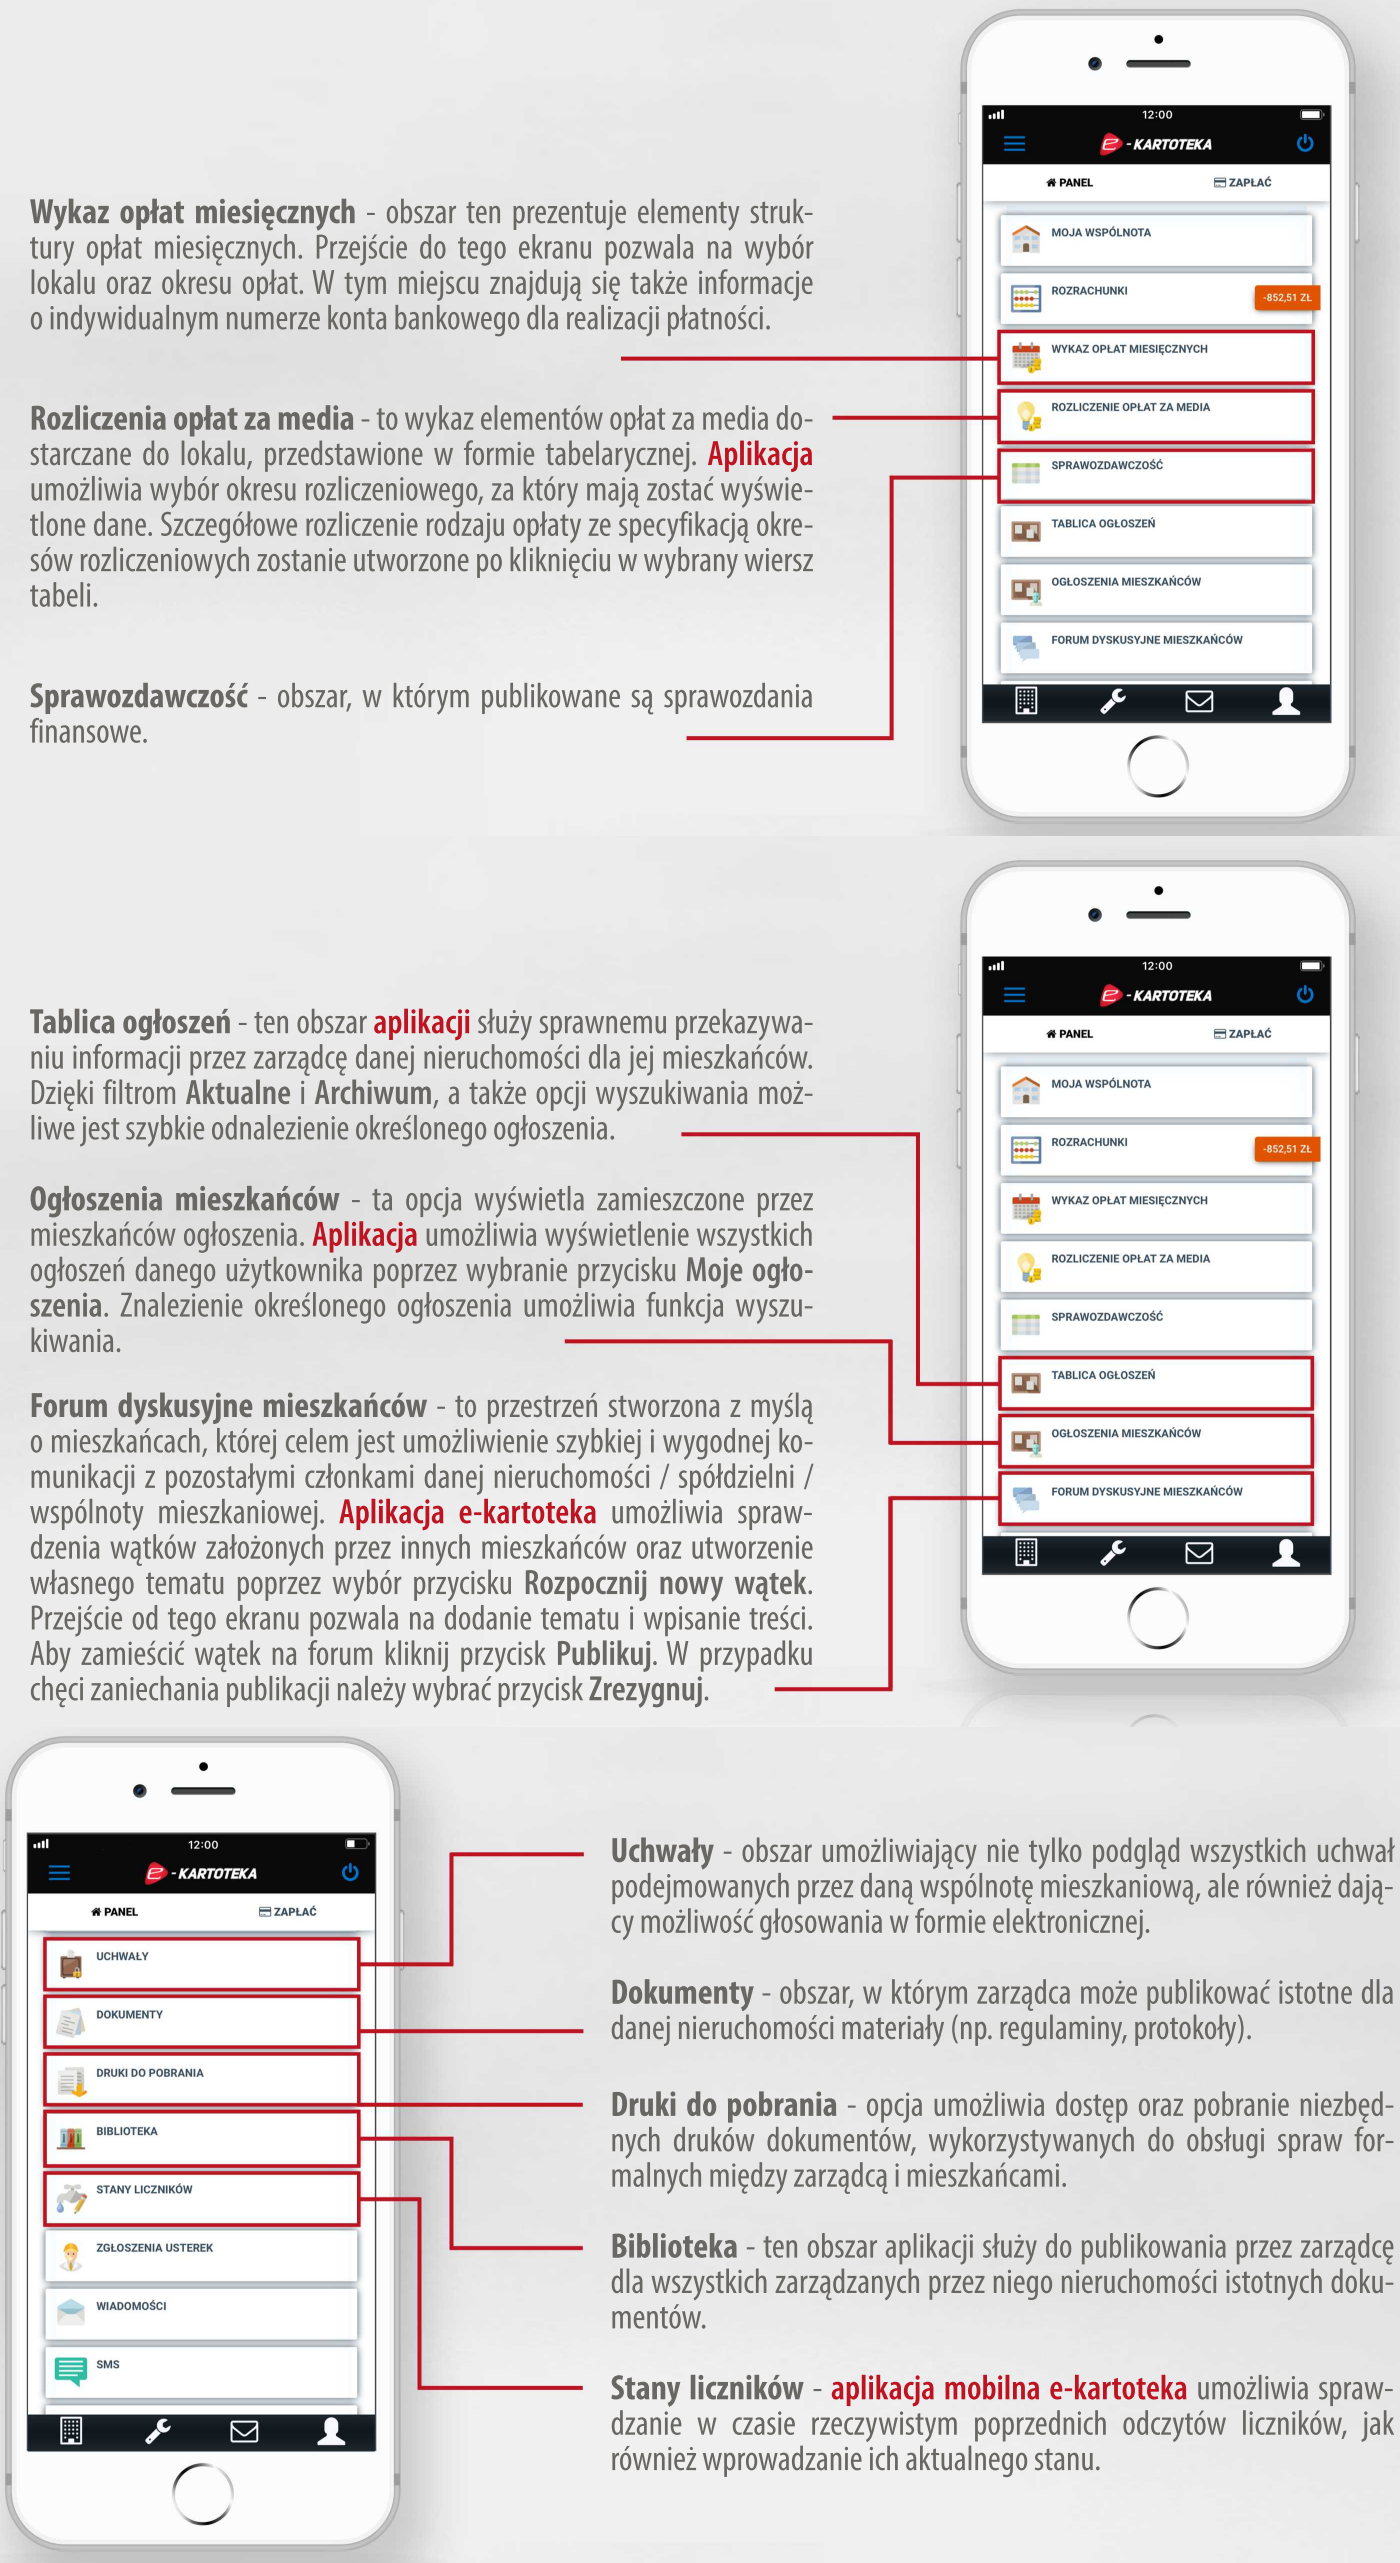
\includegraphics[width=0.6\linewidth]{zrzuty_ekranu/kartoteka_manual}
    \caption{Opis głównych funkcji oferowanych w systemie ,,e-Kartoteka''~\cite{e-kartoteka_manual}}
    \label{fig:kartoteka_manual}
\end{figure}
% TO DO: proszę uważać na apostrofy podczas cytowania - ich stosowanie w całej pracy powinno być spójne. Ja poprawiłem apostrofy w tym rozdziale na polskie pisarskie:  ,, (dolny) ''(górny) - latex zamieni dwa przecinki i dwa pojedyncze apostrofy na znaki podwójnego apostrofu dolnego i górnego.


Systemy eBOK różnią się funkcjonalnością, skalowalnością i stopniem integracji z innymi systemami, takimi jak narzędzia płatności online, systemy zarządzania nieruchomościami i aplikacje mobilne. W zależności od charakterystyki organizacji, wybór konkretnego rozwiązania będzie zależał od potrzeb operacyjnych, liczby użytkowników i stopnia automatyzacji procesów. Wdrożenie takich systemów wymaga odpowiedniego doboru technologii i architektury, co niesie za sobą wiele wyzwań. Projektowanie systemów eBOK stanowi doskonałą okazję do przetestowania i rozwijania umiejętności w zakresie programowania, automatyzacji procesów i zarządzania projektami informatycznymi. Właśnie z tego powodu podjęto się tego tematu w niniejszej pracy, by w praktyce rozwiązać problem automatyzacji obsługi wspólnot mieszkaniowych i usprawnić komunikację pomiędzy mieszkańcami a administracją.

Tematem niniejszej pracy inżynierskiej jest projektowanie i wdrożenie aplikacji Elektronicznego Biura Obsługi Klienta (eBOK) dla wspólnoty mieszkaniowej. Wybór tego rozwiązania jest odpowiedzią na rosnącą potrzebę automatyzacji procesów obsługi klienta oraz usprawnienia komunikacji między mieszkańcami a administracją. Współczesne eBOK-i nie tylko eliminują konieczność kontaktu osobistego czy telefonicznego, ale także oferują użytkownikom możliwość załatwienia większości spraw online, co wpływa na wygodę, oszczędność czasu oraz bezpieczeństwo transakcji i komunikacji.

Finalny produkt opracowywany w ramach tej pracy inżynierskiej będzie nosił nazwę ,,Harmony Home Net''. Nazwa ta odzwierciedla kluczowe cele systemu, takie jak ułatwienie komunikacji i współpracy między mieszkańcami a administracją, zapewniając przy tym płynne i zintegrowane zarządzanie nieruchomościami.


% Zwykle wprowadzenie zajmuje półtorej do dwóch stron

\section{Cel i zakres pracy}

% TO DO: podczas redakcji pracy pojawia się kłopot z czasami (przeszły, teraźniejszy, przyszły), czasownikami (dokonane, niedokonane) i trybami (orzekający, rozkazujący, przypuszczający oraz warunkowy). Zwykle podczas redagowania założeni stosuje się czasowniki niedokonane, tryp orzekający-warunkowy-przypuszczający. Proszę zwrócić na to uwagę.

Celem niniejszego opracowania jest zaprojektowanie i wdrożenie internetowej aplikacji elektronicznego biura obsługi klienta (eBOK) dla wspólnoty mieszkaniowej. Aplikacja ma ułatwiać zarządzanie procesami związanymi z komunikacją, płatnościami, zgłoszeniami technicznymi i dostępem do odpowiednich dokumentów. Dzięki temu zarówno mieszkańcy wspólnoty, jak i użytkownicy zarządzający będą mogli korzystać z kompleksowego narzędzia, które powinno automatyzować wiele codziennych zadań i zwiększać efektywność zarządzania.

Zakres prac obejmuje cały cykl rozwoju oprogramowania, począwszy od analizy potrzeb wspólnoty mieszkaniowej, przez zaprojektowanie architektury systemu, aż po wdrożenie i przetestowanie gotowego rozwiązania. Analiza wymagań będzie obejmować zarówno potrzeby funkcjonalne, jak i niefunkcjonalne, takie jak bezpieczeństwo, wydajność oraz łatwość integracji z zewnętrznymi systemami. Projektowanie ma uwzględniać iteracyjny proces testowania oraz możliwość przyszłych rozszerzeń o dodatkowe moduły funkcjonalne.

Aplikacja będzie dostępna w przeglądarce internetowej i zoptymalizowana pod kątem dostępu z różnych urządzeń, w tym również w wersji desktopowej. Backend systemu zostanie zrealizowany z wykorzystaniem technologii Java i Spring Boot, co umożliwi tworzenie skalowalnych, bezpiecznych i łatwych w utrzymaniu aplikacji. Baza danych PostgreSQL, uruchomiona w kontenerze Dockerowym, będzie stanowić fundament do zarządzania danymi.

Frontend aplikacji zostanie stworzony w języku TypeScript i frameworku Next.js, co powinno pozwolić na budowanie nowoczesnego i responsywnego interfejsu użytkownika, zapewniającego intuicyjność i szybkie działanie aplikacji.

\section{Układ pracy}
% tutaj opis zawartości kolejnych rozdziałów, można zredagować na końcu